\scanpage{96}
\figure{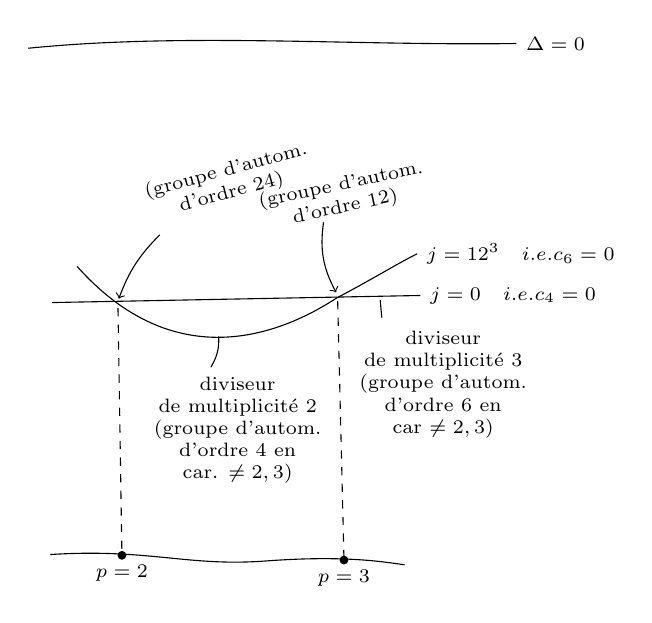
\begin{tikzpicture}[x=1cm,y=1cm,font=\scriptsize]
\draw (0,6.9) .. controls (2,7.1) and (4.1,6.93) .. (6.2,6.96) node[right] {$\Delta=0$};
\draw (0.3,3.67) -- (4.98,3.76) node[right] {$j=0\quad\text{i.e. }c_4=0$};
\draw (0.62,4.13) .. controls (1.83,2.77) and (3.14,3.22) .. (3.92,3.73)
 .. controls (4.34,3.95) and (4.68,4.16) .. (4.94,4.29)
 node[right] {$j=12^3\quad\text{i.e. }c_6=0$};
\draw[->] (1.67,4.53) to[bend right=12] (1.15,3.72);
\node[rotate=15,align=center,anchor=south west] at (1.50,4.52)
 {(groupe d'autom.\\d'ordre 24)};
\draw[->] (3.75,4.69) to[bend right=18] (3.91,3.80);
\node[rotate=12,align=center,anchor=south] at (4.08,4.64)
 {(groupe d'autom.\\d'ordre 12)};
\draw (2.42,3.24) to[bend left=16] (2.32,2.85);
\node[align=center,anchor=north] at (2.66,2.85)
 {diviseur\\de multiplicité 2\\(groupe d'autom.\\d'ordre 4 en\\car. $\ne2,3$)};
\draw (4.47,3.70) -- (4.49,3.48);
\node[align=center,anchor=north] at (5.27,3.43)
 {diviseur\\de multiplicité 3\\(groupe d'autom.\\d'ordre 6 en\\car $\ne2,3$)};
\draw[dashed] (1.14,3.60) -- (1.19,.46);
\draw[dashed] (3.93,3.69) -- (4.01,.40);
\draw (.28,.47) .. controls (1.55,.55) and (2.03,.31) .. (3.04,.39) .. controls (4.02,.46) and (4.49,.38) .. (4.78,.34);
\fill (1.19,.46) circle (1.6pt) node[below] {$p=2$};
\fill (4.01,.40) circle (1.6pt) node[below] {$p=3$};
\end{tikzpicture}}

\[
\deleted{\unsure{j}}\quad
\left\{\begin{aligned}
 \operatorname{div}(j)^+&=3\operatorname{div}(c_4)&\tfrac13\operatorname{div}(j)^+&=\operatorname{div}c_4\\
 \operatorname{div}(j)^-&=M^{(\infty)}\\
 \operatorname{div}(j-12^3)^+&=2\operatorname{div}(c_6)&\tfrac12\operatorname{div}(j-12^3)^+&=\inserted{\operatorname{div}c_6}\\
 \operatorname{div}(j-12^3)^-&=M^{(\infty)}\\
 M^{(\infty)}&=\operatorname{div}\Delta
\end{aligned}\right.
\]
\[
\left\{\begin{aligned}
 \operatorname{cl}\deleted{\unsure{\operatorname{div}}}\bigl(\tfrac13\operatorname{div}(j)^+\bigr)&=\omega^4\\
 \operatorname{cl}\bigl(\tfrac12\operatorname{div}(j-12^3)^+\bigr)&=\omega^6\\
 \operatorname{cl}(M^\infty)&=\omega^{12}
\end{aligned}\right.
\]
\hrule

Sous-site étale \inserted{$\deleted{\unsure{M}}V(c_4)=M'$} du site modulaire $\deleted{\unsure{\mathcal M}}M$ défini par l'équation $c_4=0$

a) Dans le \deleted{complémentaire} ouvert $(M'_{/6}=M'\,|\,\underbrace{(\operatorname{Spec}\mathbb Z-\{2\}-\{3\}}_{\operatorname{Spec}\mathbb Z[\frac16]})$, c'est isomorphe à $\deleted{\unsure{\operatorname{Spec}\mathbb Z[\tfrac16]}}\ B_{\mu_6}\,|\,\operatorname{Spec}\mathbb Z[\tfrac16]$ ; on peut \deleted{\unsure{se|le}} décrire \deleted{\unsure{canoniquement|comme isom.}} ces courbes \deleted{\unsure{de genre 1}}\inserted{elliptiques} sur $S$, avec $c_4=0$ (\unsure{où|si} $6$ inv. sur $S$) comme les torseurs sous $\mu_6$ ; à $E$ correspond le torseur de ses isom. avec la courbe d'équation \unsure{non} homogène $y^2=x^3+1$. [ NB. Il y a en tout $72$ courbes elliptiques sur $\mathbb Z[\frac16]$ avec $c_4=0$, car
\[
 H^1(\operatorname{Spec}\mathbb Z[\tfrac16],\mu_6)\simeq
 \deleted{\unsure{\mathbb Z_{/6\mathbb Z}\times\mathbb Z_{/6}\ \operatorname{Spec}}}
 \bigl(\mathbb Z[\tfrac16]\bigr)^*_{6}\simeq
 \mathbb Z_{/6\mathbb Z}\times\mathbb Z_{/6\mathbb Z}\times\mathbb Z_{/2\mathbb Z}
\]

b) La fibre de $M'$ en $p=2$ est de \deleted{\unsure{ordre 4}} multiplicité 4 en chaque point, en $p=3$ est de multiplicité 2. Donc $M'$ est ramifié sur $\mathbb Z$ \inserted{exactemt} en l'unique point au dessus de $p=2$ et l'unique point au dessus de $p=3$.

$M'$ est-il \uline{régulier} ?? \uuline{Non}, pas en $p=2$ \deleted{\unsure{et}}, mais régulier en $p=3$.

\smallskip\noindent\rule{.30\linewidth}{.3pt}

Sous-site étale $V(c_6)=M''$ du site modulaire.

a) Dans l'ouvert $(M''_{/6}=M''\,|\,\operatorname{Spec}\mathbb Z[\tfrac16],=M''-M''_{(2)}-M''_{(3)}$, c'est $\simeq B_{\mu_4}\,|\,\operatorname{Spec}\mathbb Z[\tfrac16]$.

(il y a $\unsure{-|=}$32 \unsure{courbe|courbes} elliptiques avec $c_6=0$ sur $\mathbb Z[\frac16]$, qu'on peut choisir comme origine \ldots)

b) $M''_{(2)}$ est de multiplicité 6, $M''_{(3)}$ est de multiplicité 3, Donc $M''$ est ramifié sur $\mathbb Z$ \unsure{exactemt} en l'unique pt sur $p=2$ et l'unique point sur $p=3$.

$M''$ est-il régulier ?? \uuline{Non}, pas en $p=2,3$ !
% archive sheet number: 95
